\begin{comment}
	\pagebreak
\end{comment}

\section{Generative Adversarial Networks}
\textbf{Imperfect Model:} High LL can result in bad samples and vv\\
memorise training data (-LL), high noise samples (+LL)\\
\begin{comment}
	\textbf{Question:} Is likelihood a good indicator for the quality of samples?\\
	It has been shown that with imperfect models a high likelihood does not imply good sample quality.\\
	\textbf{Approach:} Do not try to model denisity explicitely\\
	
	\begin{Figure}
 		\centering
 		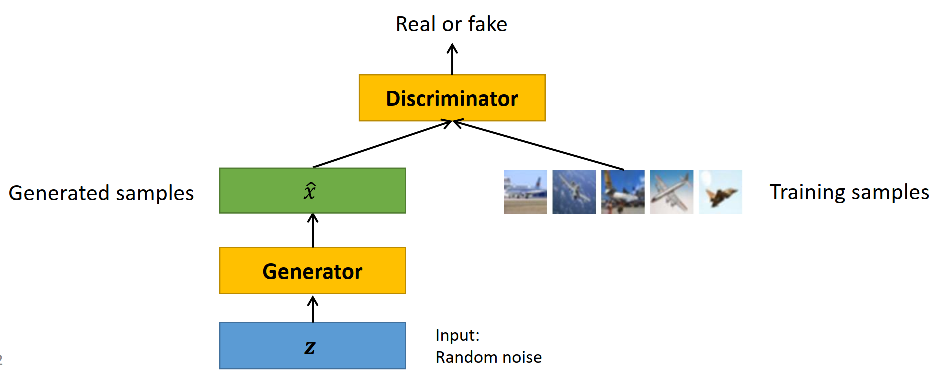
\includegraphics[width=\linewidth]{graphic/gan-intuition}
 		\captionof{figure}{GAN Intuition}
	\end{Figure} 
\end{comment}

\textbf{Generator:} map $z \in \R^Q$ to observ. $x \in \R^D$, $G: \R^Q \rightarrow \R^D$\\
\textbf{Discriminator:} trained on $\whx$ and $x$, $D: \R^D \rightarrow [0,1]$\\
No markov chain necessary\\
\begin{comment}
	The discriminator can be thought of as learned loss-function.
\end{comment}

\textbf{Loss:}$-\frac{1}{2N}(\sum_i^N (y^{(i)}) \log(D(x^{(i)})) + \sum_n^{2N} (1 - y^{(i)}) \log(1 - D(x^{(i)})))$\\

\textbf{Train:} $G^*, D^* = \argmin_G \argmax_D \log(D(x)) + \log(1-D(\whx))$\\
\textbf{Opt:} $V(G, D^*) = \E_{x \sim p_d}(\log(D^*(x))) + \E_{x \sim p_m}(\log(1-D^*(x))) \\
= -\log(4) + 2 D_{JS}(p_d(x) || p_m(x))
= -\log(4)$ if $p_d(x) = p_m(x)$\\
\begin{comment}
	We can use various NN's for G and D
	
	\begin{Figure}
 		\centering
 		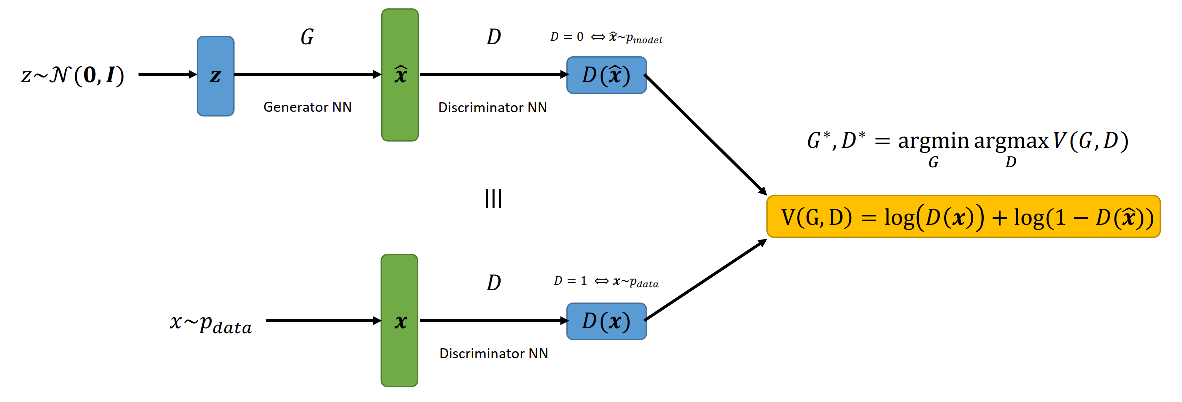
\includegraphics[width=\linewidth]{graphic/gan-arch}
 		\captionof{figure}{GAN Architecture}
	\end{Figure}
\end{comment}

$f(x) = a \log x + b \log (1-x) \in [0,1]$ has max at $\frac{a}{a+b}$\\

\textbf{Update D:} for $k: \nabla_{\Theta_D} \frac{1}{N} \sum \log(D(x^{(i)})) + \log (1 - D(G(z^{(i)})))$\\
\textbf{Optimum} $D^* = \frac{p_{data}(x)}{p_{data}(x) + p_{model}(x)}$\\
\begin{comment}
	\Note{We are using gradient ascent here, because D wants to maximize the loss function}\\
\end{comment}

\textbf{Update G:} $\nabla_{\Theta_G} \frac{1}{N}\sum \log(D(G(z^{(i)})))$ (ascent)\\
\begin{comment}
	\Note{We are also using gradient ascent here with a changed objective, instead of using descent on $\log(1 - D(G(z^{(i)})))$, because it has better gradient properties.}\\ 
	
	\begin{Figure}
 		\centering
 		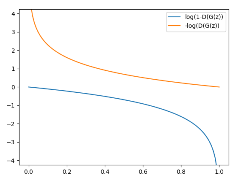
\includegraphics[width=\linewidth]{graphic/gan-g-obj}
 		\captionof{figure}{GAN Generator objective}
	\end{Figure}
\end{comment}

\textbf{Assumption:} capacity, $D \rightarrow D^*$, opti. $p_{model}$\\
\begin{comment}
	G and D have enough capacity, descriminator reaches $D^*$ in every outer iteration, we optimize $p_{model}$ instead of parameters of the model\\
\end{comment}

\textbf{Mode Collapse:} $G$ finds one mode, $D$ fails to reject\\
\begin{comment}
	This reduces the set of generated examples, since G has a gold-shitting donkey. 
	If D doesn't figure out to reject it, the next iteration of G again uses it.

	Unrolling is updating the parameters of D in the first step, while adjusting the parameters of G at the k'th step.
	G is looking k steps ahead on how D is reacting, and generates the gradient on each step of the way.
	Computationaly, we are backpropagating the gradient of G through all k steps, as in LSTM's.\\
	
	\begin{Figure}
 		\centering
 		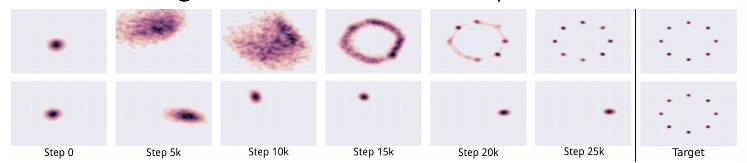
\includegraphics[width=\linewidth]{graphic/gan-mode-collapse}
 		\captionof{figure}{GAN Mode collapse}
	\end{Figure}
\end{comment}

\textbf{Oscillation:} limited capacity and not $D^*$\\

\textbf{Wasserstein:} work to similarity; +no collapse, +stable\\

\textbf{Cons:} no explicit $p(x)$, nor sample LL, carful balancing, less theory\\ 



